% ED26-BM-RAT2021-13-3: Knauff, MIT2021, chapter13.3, pp.735--744.
\chapter{Visualization and Rationality}
\label{sec:p19-rationality-13-3}

A picture can expose a relation, suggest a proof, distract from a relation,
or create a vivid experience without supplying a valid conclusion. Knauff's
chapter asks about these different contributions to epistemic rationality.
Its organizing distinction is between external visual aids and internal
picture-like imagery, with a further distinction between pictorial detail
and abstract spatial organization. The evidence concerns particular
reasoning, learning and representational tasks, not an unconditional rule
that more visualization improves rationality
\parencite[pp.~735--744]{Knauff2021VisualizationRationality}.
\index{visualization!external and internal}\index{visual impedance effect}
\index{spatial representation!distinct from visual detail}

The chapter combines philosophical examples, cognitive experiments,
neuroimaging and computational explanations. These supply different kinds
of warrant. A valid geometrical argument is not a measured learning effect;
slower responses are not the same as more invalid responses; an activation
contrast is not a proof of the content of a mental representation; and a
simulation reproducing behavior does not uniquely identify its human cause.

\section{Representations, tasks and standards of success}
\label{sec:p19-rat133-distinctions}

\begin{hbdefinition}{def:p19-rat133-visualization}{External aids, internal images and spatial organization}
\emph{External visualization} is a presented picture, graphic or diagram
intended to help a reasoner acquire or use information. \emph{Internal
visualization}, in this chapter's narrower sense, is picture-like mental
imagery experienced as analogous to visual perception. A \emph{spatial
representation} instead preserves a layout, order or relation while possibly
omitting color, texture, detailed shape or a viewpoint-specific appearance.
Spatial organization does not require a consciously experienced mental picture.

An external drawing can elicit internal imagery, but the two are not the
same object or manipulation. Visually presented premises can be processed
abstractly; verbally presented premises can elicit vivid imagery. Comparing
display formats therefore does not, by itself, isolate an internal process.
\end{hbdefinition}

Knauff uses epistemic rationality for belief acquisition, formation and
revision guided by appropriate normative standards. Logical consequence is
one benchmark for deduction, not an assertion that classical logic is the
right standard for every everyday inference. Remembering a scene, rotating
an object, learning from a display and judging whether a conclusion follows
are distinct tasks even when they all involve pictures
\parencite[pp.~735--736]{Knauff2021VisualizationRationality}.

\begin{hbdefinition}{def:p19-rat133-success}{Four questions that a successful display does not collapse}
\begin{enumerate}
\item \emph{Representational adequacy}: does the display encode the relevant
      premises without adding unstated information or hiding alternatives?
\item \emph{Inferential validity}: does the conclusion follow under the
      declared interpretation and assumptions, rather than merely hold in
      one drawn arrangement?
\item \emph{Task performance}: how accurately and quickly do specified
      participants answer the specified question with that representation?
\item \emph{Transfer}: does a benefit persist on new materials, populations,
      unaided tasks or delayed tests, rather than only the trained display?
\end{enumerate}
A convincing appearance, subjective vividness or correct response on one
trial answers none of the other questions automatically.
\end{hbdefinition}

The distinction complements the declared set-diagram semantics in
\cref{def:p12-r131-region-reading}: physical area there has no set-cardinality
meaning. It also complements the possibility/necessity distinction in
\cref{def:p19-rat132-task}: a preferred arrangement is not every
arrangement allowed by the premises. Here the question is which properties
of a representation help or impede people in performing such tasks.

\section{External visualization: the midpoint-square example}
\label{sec:p19-rat133-external}

Knauff's first mathematical example places an inner square at the midpoints
of an outer square's sides. The drawing suggests folding the four corner
triangles inward and seeing why the outer area is twice the inner area.
The qualification is crucial: a rough drawing can suggest a relationship
without establishing the exact midpoint and square conditions
\parencite[p.~736, fig.~13.3.1]{Knauff2021VisualizationRationality}.

\begin{figure}[htbp]
\centering
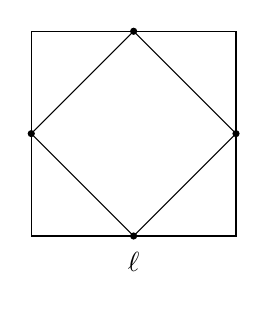
\begin{tikzpicture}[x=1.3cm,y=1.3cm]
\draw (0,0)--(2,0)--(2,2)--(0,2)--cycle;
\draw (1,0)--(2,1)--(1,2)--(0,1)--cycle;
\fill (1,0) circle (1.3pt); \fill (2,1) circle (1.3pt);
\fill (1,2) circle (1.3pt); \fill (0,1) circle (1.3pt);
\node at (1,-.25) {\(\ell\)};
\end{tikzpicture}
\caption{An independently drawn schematic of the source's midpoint-square
problem. The marked points are stipulated midpoints; the picture's physical
size is not the premise establishing the area relation.}
\label{fig:p19-rat133-midpoint-square}
\end{figure}

\begin{hblemma}{thm:p19-rat133-square-area}{proved=annex:p19.rat133-square-area}{Area ratio under exact Euclidean assumptions}
For a Euclidean square of side \(\ell>0\), joining consecutive side
midpoints forms a square. If \(A_{\mathrm{out}}\) and
\(A_{\mathrm{in}}\) are respectively the outer and inner areas, then
\[
             A_{\mathrm{out}}=\ell^2,
\qquad       A_{\mathrm{in}}=\ell^2/2,
\qquad       A_{\mathrm{out}}=2A_{\mathrm{in}}.
\]
The conclusion is general over the stipulated squares, not inferred from
measuring the schematic or a participant's impression.
\end{hblemma}

The diagram's epistemic role can thus be discovery or understanding of an
argument whose conditions are justified separately. Knauff reviews contrasting
mathematical attitudes, associating imagination with Klein and independence
from particular figures with Hilbert. These are attributed positions, not a
proof that visual reasoning is either universally legitimate or universally
unreliable. His discussion of Euler, Venn, Peirce's iconicity and Shin's
formal diagram work likewise distinguishes a formal visual language from an
unregulated inspection of an appealing image
\parencite[pp.~735--736]{Knauff2021VisualizationRationality}.

\subsection{Different external displays can have opposite effects}

Knauff reports Bauer and Johnson-Laird's comparison of sentence-only
conditional problems with conditions also supplied with abstract line diagrams
clarifying logical relations. He reports better performance with those
diagrams. In contrast, his account of Hyperproof studies connects stronger
visualizing tendencies and weaker logic skills with potential benefit from
learning more abstract strategies. Neither report establishes that a learner's
initial preference identifies the most effective format
\parencite[pp.~736--737]{Knauff2021VisualizationRationality}.

Further survey examples compare photographs of real objects with more
abstract, annotated objects in a virtual environment for conditional
reasoning, and discuss route descriptions and photorealistic navigation.
The proposed explanation is that irrelevant detail can compete with
information required by the inference. Multimedia redundancy and seductive
details are neighboring hypotheses: an eye-catching addition can distract
from meaningful learning rather than enhance it. These are distinct tasks
and mechanisms, not one pooled visualization effect
\parencite[p.~737]{Knauff2021VisualizationRationality}.

For these external-display studies the chapter gives qualitative task and
format descriptions but not complete recruitment records, analysis samples,
effect estimates or uncertainty intervals. Their reported directions are
retained as survey claims, not independently quantified here. In particular,
the evidence does not warrant excluding all illustrations, adding all
diagrams, or generalizing one navigation or instructional result to every
logical task. The relevant question is what each representation encodes
and what processing the comparison condition requires.

\section{Internal imagery and the visual impedance hypothesis}
\label{sec:p19-rat133-impedance}

Knauff reviews the imagery debate through historical philosophical positions,
scientific introspection, the W\"urzburg school's reports of imageless
thinking, behaviorist criticism and the later return of representational
accounts. Boltzmann's theoretical imagery and Kekul\'e's reported inspiration
for a cyclic benzene structure are scientific anecdotes, not controlled
evidence that imagery caused discovery or is necessary for deduction.
Perky's imagery/perception confusion and Kosslyn and colleagues' remembered-
island scanning task address other questions: in the latter, response time
to move mentally between landmarks was reported to track map distance.
That does not establish how people validate a logical conclusion
\parencite[pp.~737--738]{Knauff2021VisualizationRationality}.

The visual impedance hypothesis concerns visual detail irrelevant to an
inference. It predicts that selecting the relevant relation from a vivid
picture can add processing, whereas an abstract layout may encode that
relation directly. The contrast is not between sensation and no cognition,
or between images and language as exclusive media.

The competing propositional account treats reasoning as operating on a
language of thought, with visual imagery potentially an epiphenomenon rather
than the inferential medium. Knauff presents the imagery debate as unresolved,
while arguing that content-sensitive interference challenges a simple
picture-inspection account. A formal proof written in sentences does not
show that its human solver used sentence-like internal representations;
likewise, the experience of a picture does not show that the picture performed
the inference \parencite[pp.~736,738]{Knauff2021VisualizationRationality}.

\begin{hbdefinition}{def:p19-rat133-four-classes}{Operational imagery and spatial ratings}
The chapter distinguishes four relation-material classes:
\begin{center}
\begin{tabular}{lll}
Class & Easy to envisage visually & Easy to envisage spatially\\ \hline
visuospatial & yes & yes\\
visual & yes & no\\
spatial & no & yes\\
abstract/control & no & no
\end{tabular}
\end{center}
These are classifications under a rating procedure, not intrinsic immutable
properties of words or people. Above/below can suggest a spatial order;
cleaner/dirtier can elicit pictorial detail not needed to compare positions
on an abstract scale. The original experiments call their low-visual,
low-spatial comparison materials \emph{control relations}; the 2021 chapter
also calls that class abstract.
\end{hbdefinition}

\subsection{The original 2002 experiments: measures and boundaries}

Knauff and Johnson-Laird first asked ten native-English-speaking Princeton
student volunteers to rate assertions on separate seven-point visual and
spatial scales. They identified visuospatial, visual and control relation
pairs, controlling word frequency and swapping the same animal nouns. An
initial German norming study with twelve Freiburg students still did not
isolate purely spatial pairs. A later twenty-student bipolar visual/spatial
rating procedure selected north/south and ancestor/descendant materials.
Thus the four-class description emerged through different norming procedures;
it is not a single successful orthogonal manipulation of two independent
subjective scales \parencite[pp.~364--368]{KnauffJohnsonLaird2002VisualImpedance}.

\paragraph{Participants, tasks and comparisons.}
Experiment~1 tested 22 Princeton undergraduates for course credit, mean age
19.5, twelve female and ten male. Each evaluated 24 randomly ordered
three- or four-term transitive inferences using visual, visuospatial or
control relations; half the proposed conclusions were valid.
Experiment~2 used twenty new students from the same population, 24
conditional/transitive problems, and four arrangements of a relation and
its converse to manipulate difficulty. Experiment~3 tested 24 Freiburg
undergraduates, mean age 22.4, fourteen female and ten male, paid or given
credit. They evaluated 32 three- or four-term problems with all four classes
using German spatial expressions
\parencite[pp.~365--368]{KnauffJohnsonLaird2002VisualImpedance}.

All were within-participant comparisons. Premises appeared separately in
black text, then a proposed conclusion in red; presentation was self-paced.
Participants judged necessary consequence with keyboard responses after
four practice problems. The computer recorded premise-reading times,
answers and conclusion-response latency. These were verbally specified
relations, not comparisons between showing and withholding external pictures.
No probability-recruitment frame or prospective power calculation is reported.

\begin{table}[htbp]
\centering\small
\begin{tabular}{lrrrr}
 & visual & control & visuospatial & spatial\\ \hline
Exp.~1 correct (\%) &86&92&90&\text{not tested}\\
Exp.~1 correct-response \(\mathrm{RT}\) (s)&2.65&2.38&2.20&\text{not tested}\\
Exp.~2 correct (\%)&77&67&68&\text{not tested}\\
Exp.~2 correct-response \(\mathrm{RT}\) (s)&3.37&2.64&2.46&\text{not tested}\\
Exp.~3 correct (\%)&73&78&72&72\\
Exp.~3 correct-response \(\mathrm{RT}\) (s)&4.48&3.81&3.74&3.52
\end{tabular}
\caption{Original 2002 Table~2 summaries. Latencies concern correct
responses, not all responses or a separately observed imagery-operation
duration. The article supplies no confidence intervals for these cell means.}
\label{tab:p19-rat133-original-outcomes}
\end{table}

In each experiment, visual relations reliably slowed correct responses.
Experiments~1 and~2 report visual-versus-control Wilcoxon comparisons of
\(z=3.07,p<.002\) and \(z=2.46,p<.02\), respectively; Experiment~3
reports visual slowing relative to the other three classes
\((z=2.46,p<.015)\).
The predicted latency order was supported, but the direct visuospatial or
spatial speedups over controls were not significant. Accuracy differences
among relation classes were not significant in any of the three experiments.
The original supports visual latency impedance, not the claim that these
same experiments demonstrated more reasoning errors or an established
pure-spatial advantage \parencite[pp.~365--369]{KnauffJohnsonLaird2002VisualImpedance}.

Reading and conclusion times must also be distinguished. Experiment~3's
spatial premises took relatively long to read, particularly the less frequent
north/south terms, despite the low conclusion latency in that condition.
The authors discuss frequency, interpretation of transitivity and plausibility
as alternative influences. They balanced converse relations and fixed nouns,
but such controls do not turn introspective ratings into a direct measurement
of the mediating representation. The samples are small student cohorts;
the language and material differences limit transfer between experiments
and beyond their tasks \parencite[pp.~368--370]{KnauffJohnsonLaird2002VisualImpedance}.

The 2021 chapter's broader accuracy claim cites other work as well, rather
than being discharged by the 2002 study alone. It also reports individual
differences based on verbalizer--visualizer questionnaires, reading-deficit
groups, congenitally blind participants and minimally invasive surgery
training. Those findings concern different populations, measures and tasks;
they are not replications of one shared numerical effect
\parencite[pp.~738--739]{Knauff2021VisualizationRationality}.

\section{Neural evidence: distinguish phases, contrasts and interpretations}
\label{sec:p19-rat133-neural}

Knauff reports a distributed frontal, temporal and parietal reasoning network,
with additional visual-region activity for some imagery-provoking materials.
The chapter's Figure~13.3.2 distinguishes premise processing, integration
and conclusion evaluation. Its phase rows display cortical activation patterns,
not the visual content of thought, rates of correct inference or proof that
any one region alone implements rationality
\parencite[pp.~739--740]{Knauff2021VisualizationRationality}.

\paragraph{The original 2006 record behind the figure.}
Fangmeier and colleagues tested twelve right-handed male undergraduate and
graduate students, mean age 22.4 (SD 1.98), with normal or corrected vision
and no reported neurological/psychiatric disorder or significant drug abuse.
They used 32 spatial reasoning problems and 32 matched maintenance problems
in four pseudorandomized scanner runs. Premises and queries were sequences
of letters \(V,X,Z\) placed left or right of the screen center rather than
ordinary-language sentences. The reasoning response judged whether a new
relation followed; the maintenance response judged whether the query
repeated a previous premise. Pre-scanner training used twelve problems to
reach at least 75\% accuracy
\parencite[pp.~321,330--332]{FangmeierEtAl2006ThreeStage}.

Each letter appeared for 1500~ms, followed by another letter for 1500~ms
and a 1000-ms pause; each premise or query thus occupied 4000~ms.
The design sought to hold visual material and memory load fixed while
contrasting integration/validation demands. Responses used an MRI-compatible
box. The study measured response accuracy and latency, event-related BOLD
signals and a post-scan Block Design Test. The behavioral comparison was
91\% correct for reasoning versus 97\% for maintenance
\((Z=2.31,p=.021)\), with mean latencies 3021 versus 2843~ms
\((Z=-2.04,p=.041)\). No confidence interval for these differences is
printed \parencite[pp.~322,330--332]{FangmeierEtAl2006ThreeStage}.

The original describes early \emph{occipito-temporal and visual association}
activity, anterior prefrontal involvement in integration, and prefrontal
plus posterior-parietal activity in validation. This is the anatomical
scope of the OTC labels in the chapter figure, not a demonstrated V1-only
or primary-visual-cortex result. Reasoning-minus-maintenance contrasts
identified greater anterior-prefrontal activity in the second phase and
prefrontal/right-precuneus activity in the third. They do not show that
every other region is inactive or that inference occurs only after premise
integration \parencite[pp.~322--330]{FangmeierEtAl2006ThreeStage}.

The analysis used correct trials, SPM99 random-effects comparisons, a
height threshold \(t=3.0\) and cluster-level multiple-comparison correction
for reported within-condition clusters. An additional response-time regressor
addressed task-difficulty differences without removing the reported central
contrasts. The published methods specify different within-phase and
between-condition contrasts; a thresholded map is not a direct movie of
three isolated mental operations. The sample was all male, right-handed,
student volunteers, with Block Design scores in a restricted normal-to-
superior range. Reverse inference from a region to a unique representation,
selection of only correct trials and unequal task difficulty remain material
interpretative limits. The authors themselves caution that other problem
types can elicit other processes
\parencite[pp.~322--330,332]{FangmeierEtAl2006ThreeStage}.

\begin{proofboundary}{def:p19-rat133-clinical-boundary}{Survey extensions are not treatment, diagnosis or etiology}
The chapter reports visual-cortex TMS facilitating some reasoning tasks and
parietal TMS impairing others, and interprets a blind-participant comparison
as evidence against a need for pictorial imagery. It also mentions lorazepam,
autism-related reports and reading-deficit studies. These are not all the
same manipulation or population. The chapter does not provide the complete
sample/design/intensity/control/effect/uncertainty record for each, and those
original studies are not independently quantified in this entry.

In particular, a reasoning-performance comparison involving dyslexic readers
does not by itself establish that imagery is a main cause of dyslexia; that
strong etiological suggestion in the survey is not adopted here. An
autobiographical report, questionnaire grouping or congenital-blindness
comparison does not randomly assign a mental representation. Neither a
drug nor a TMS report is a recommendation to intervene to improve reasoning.
Grandin's \emph{Thinking in Pictures} is the source's autobiographical
illustration of helpful visual practice alongside difficulty with abstraction,
not a controlled estimate for autistic people generally.
\end{proofboundary}

This preserves the chapter's reported contrasts without promoting them
to universal clinical or causal conclusions
\parencite[pp.~735,738--739]{Knauff2021VisualizationRationality}.

\section{Computational explanations and the preferred-model boundary}
\label{sec:p19-rat133-models}

Knauff's computational examples distinguish a display or image-processing
program from an explanation of human inference. WHISPER manipulated
blocks-world diagrams; Kosslyn and Shwartz used metrically located contents
in filled/unfilled matrix cells. Berendt's imagery model reconstructed some
preferences for interpretations of ambiguous premises, while Schlieder's
more parsimonious representation retained the ordering of endpoints rather
than extensive visual detail. The comparison asks which information and
operations are needed to reproduce a specified response pattern, not which
picture looks most natural \parencite[p.~740]{Knauff2021VisualizationRationality}.

PRISM represents tokens in an abstract spatial array with a movable focus,
construction, inspection and variation operations. A preferred model can
support a quick answer while omitting other satisfying arrangements.
The actual original implementation and its limits are treated in
\cref{sec:p19-rat132-prism}: its descriptive search policy does not routinely
seek a counterexample to a query already true in the preferred model, and
its defaults are not every proposed working-memory limitation.
Thus an erroneous necessity judgment can be modeled without declaring it
logically valid. The 2021 visualization chapter also points to preliminary
computational simulations of impedance, explicitly leaving algorithmic
details open \parencite[pp.~740--741]{Knauff2021VisualizationRationality}.

\section{Corollaries, comparisons and task lookup}
\label{sec:p19-rat133-lookup}

Knauff's six concluding claims form an argument with distinct evidential
strengths. First, introspection can misidentify the process producing an
answer. Second, a descriptive theory must explain errors as well as
normatively successful answers. Third, he argues that imagery can causally
impede inference, proposing a detour through visual processing before
abstract relational work; the particular detour is an explanatory hypothesis,
not a uniquely identified algorithm. Fourth, imagery's educational value
depends on task and representation rather than vividness alone. Fifth,
external detail can elicit internal imagery, making relevance and overload
important. Sixth, logical reasoning is a special domain, so transfer to all
thinking is not established \parencite[p.~741]{Knauff2021VisualizationRationality}.

\begin{hbmethod}{def:p19-rat133-evaluate-aid}{Evaluate the representation against its actual reasoning task}
\begin{enumerate}
\item Fix the query and correctness criterion: memory, identity under rotation,
      feature binding, possibility, necessity, learning or proof.
\item Specify the encoding, viewpoint, scales and incidental visual features.
      Separate external format from any hypothesis about internal imagery.
\item Check whether a proposed inference is warranted by the encoded premises,
      including alternatives not displayed in a preferred arrangement.
\item Compare representations with declared participants, materials, controls
      and instructions. Measure accuracy, reading/encoding time and response
      latency separately when the explanation depends on that distinction.
\item Report uncertainty, negative as well as positive comparisons, and
      possible confounds such as language, semantic content, word frequency,
      prior skill, speed--accuracy tradeoffs and difficulty.
\item Test transfer rather than inferring it from appeal, preference or local
      success. A new population or unaided task is a new evidential question.
\end{enumerate}
This procedure implements the representational and evidence distinctions
above; it is not a theorem that abstract displays always outperform concrete
ones. The evidence-reporting interface is \cref{def:p19-evidence-record}.
\end{hbmethod}

A successful lookup use identifies why the midpoint diagram suggests a
general relation and supplies the exact geometrical justification, or
interprets the 2002 latency effect under its actual materials and samples.
A failed use infers universal validity from one pleasing picture, treats
slowing as automatically more errors, infers V1 or an exact mental algorithm
from a thresholded association map, or claims general rationality training
from a local display benefit.

Logical diagrams in \cref{sec:p12-rationality-13-1} have declared syntax,
semantics and proof obligations; this chapter studies assistance and
interference in using representations. Spatial/temporal reasoning in
\cref{sec:p19-rationality-13-2} concerns relational constraints and
preferred-model procedures; this chapter separates those abstract relations
from pictorial detail. Mental rotation in \cref{sec:p19-mental-rotation}
compares geometric identity responses across disparities, while its
feature-binding studies measure retention of color-to-part correspondences
during transformation. Neither is the 2002 necessary-consequence task or
the 2006 reasoning-versus-maintenance contrast. Compatible findings across
these tasks can constrain explanations without becoming one common
visualization effect or a universal measure of rationality.
